\chapter{Architecture} \label{CH:architecture}

\section{Architectural Overview}\label{sec:arch:overview}
The goal of the Torchbearer system is simple: given the latitude, longitude and approach bearing of a maneuver point, render a string describing the most salient landmark at that location. The problem which Torchbearer solves can be expressed as simply

\begin{equation}\label{eq:problem}
    f(lat, long, bearing) \longrightarrow landmark
\end{equation}

where $f$ is some method of landmark selection and description. The Torchbearer system provides multiple implementations of $f$, which we call pipelines. Each pipeline consists of an ordered set of tasks, $T$. Each task $t_i \in T$ accepts some input from the previous task $t_{i-1}$ and returns some output to be input to the next task $t_{i+1}$---the obvious exceptions being the first task, which takes a tuple $(lat, long, bearing)$ as input, and the last task, which outputs the selected landmark, inclusive of description---the final result of the pipeline. Each task progressively solves a small part of the landmark selection problem, such that at the end of the pipeline a lexical description of the most suitable landmark has been determined. It is natural to consider a pipeline as a composition of functions:

\begin{equation}\label{eq:pipeline}
    P=t_{n-1} \dots t_1(t_0(lat, long, bearing)) \longrightarrow description
\end{equation}

where $n \equiv \mid T \mid$. As an implementation detail, it is important to note that tasks can be performed in parallel if they all take the same input form the previous task. Examples of such parallelization will be seen in the descriptions of each specific pipeline.

\section{Input and Output}\label{sec:arch:io}
In general, a task receives a tuple $X$ as its input and yields a tuple $Y$ as its output. A task’s output must be inclusive of its inputs, that is, $X \subset Y$. Let $p_+ = Y \setminus X$, then $p_+$ is the context contribution of a given task--the information which that state has added to the pipeline's overall knowledge, or state. A task does not necessarily need to make a context contribution--some tasks perform important functions that do not lend any additional knowledge directly, but rather complete operations which are  prerequisites for future tasks (such as downloading an image).

It is important to note that each task has a binding contract in terms of its input and output, based on where it sits in the pipeline. For example, task $t_1$ must accept input corresponding to the output of task $t_0$, and must provide output corresponding to the input to task $t_2$. This presents a not insignificant constraint in regards to rearranging tasks within a pipeline: even if $t_1(t_2) == t_2(t_1)$ (that is, the order in which the pair of tasks is executed is not important) the two tasks could not change positions in the ordered set of tasks for the pipeline unless their inputs and outputs were identical. 

\section{Orchestration}\label{sec:arch:orchestration}
In order to implement the function composition approach discussed above, each pipeline requires a system to progress a maneuver point through each task in the pipeline. We call such a system the pipeline’s \textit{Orchestrator}. The Orchestrator is the manifestation of the pipeline, in the sense that it is solely responsible for the intake of new maneuver points to be processed and overseeing the ordered execution of each task for that maneuver point.

The Orchestrator is centralized service which acts as a specialized message broker. For each task $t$ in the pipeline, the Orchestrator maintains a FIFO queue $q_t$ of maneuver points needing to be processed through that task. Queue items are tulpes containing the unique identifier of the maneuver point, a token representing the specific task instance and the input to the given task, $I_t$.

A task \textit{worker}, described in the next section, polls the Orchestrator for a task in need of completion; if such a task is available it is popped from queue and returned to the worker. (Polling is discussed in greater detail in the following section.) When the worker has the completed the task, it sends the results back to the Orchestrator, which then adds a new item to the queue corresponding to the next task $t_+$, including the output of $t$ (which is the input to $t_+$). If the execution of the task resulted in an error, this is sent to the Orchestrator, which then halts further execution of the pipeline for that maneuver point.

The Orchestrator supports parallel execution of tasks: a maneuver point can be placed into two queues simultaneously, and progression of the pipeline paused until \textbf{both} tasks complete. The input $X$ to the next task $t+1$ is then the union of the outputs of the $n$ parallel tasks:

\begin{equation}\label{eq:paraOrch}
    X_{t+1} = Y_0 \cup Y_1 \dots \cup Y_n
\end{equation}

An Orchestrator also maintains a database of pipeline state, including, for each maneuver point, the output of each task, or error details if one occurred. This allows the execution for a specific point to be traced or monitored throughout the pipeline.

\section{Task Implementation}\label{sec:arch:pipeline_imp}
A task is solved by a worker. A worker is an independent, isolated computational entity which is responsible for the execution of a specific task. There can be any number of (identical) workers for a task active at one time, essentially functioning as a cluster which allows for multiple instances of the given task to be executed simultaneously. (Each instance of a task will only be run on one worker.)  Workers are stateless: in order to complete its task, a worker relies only on the input it receives from the Orchestrator, without regard to previous tasks completed by other workers. Workers have no awareness of the context in which they do their jobs, in the sense that workers can handle tasks from multiple pipelines and do not care about the order in which they are asked to handle tasks. 

A worker performs three essential functions: first, it polls (a) pipeline Orchestrator(s) to be alerted of new tasks needing execution. Second, it carries out the computational operations needed to complete the task, utilizing inputs provided by the Orchestrator. Lastly, it returns outputs to the Orchestrator upon successful completion of the task, or alerts the Orchestrator of a failure. 
 
\subsection{Polling for Tasks}
The first function of a worker is to poll pipeline Orchestrators for tasks in need of completion. A worker will ask only for the task it is meant to perform. It is important to note that task assignment is based on a pull mechanism, as opposed to a push mechanism: rather than Orchestrators routing tasks to specific Workers, each Worker is responsible for “finding” its own work by asking Orchestrators for available jobs. While an Orchestrator serves as a manager for tasks, having state related to the precise status of all pending tasks in its pipeline, it does not serve as a manager for Workers. Indeed, no component of the Torchbearer system maintains state related to the Worker pool. This allows workers to be stood up or fail without disruption.

The polling mechanism is contained within its own thread and runs in a continuous loop. Each iteration of the loop consists of the following: to initiate the polling sequence, a Worker sends an HTTP GET request to the Orchestrator. If the Orchestrator has any tasks the worker is capable of completing, it immediately responds with a payload containing a list of tuples, where each tuple contains inputs and a unique identifier corresponding to each specific task. If no such task is currently available, the Orchestrator holds the request open for up to 60 seconds, waiting for a task to become available. As soon as a task becomes available the payload is sent and the request ended. If no task becomes available during the 60 second window, the request is terminated with an empty response.

When a worker receives a response from the polling request, it first checks to see if the response contains a payload (indicating that at least one task was received.) If a payload is present, it spawns a thread for each received task to process (complete) the given task, passing in the input and unique identifier received from the payload. If no payload is present, no further action is taken. The current iteration of the polling loop is complete, and the process repeats with a new polling request immediately being invoked.

\subsection{Task Execution}

The approach to solving or completing the worker’s task is contained in the execution step. The majority of this step’s procedure is dependent on the task, and will be discussed for each task in depth later on. It is important at this juncture to understand only that the execution step for a given task runs asynchronously in its own thread, spawned by the polling thread and being provided with both the inputs to the task and unique identifier of the task. The runnable routine of this thread consists of a program which will accept the task’s inputs and yield the task’s outputs--that is, it solves or completes the task. 

\subsection{Submitting Results}

If the task completes successfully, an HTTP POST request is sent by the task execution thread to the Orchestrator, consisting of task token as well as the yielded output. If any error occurred during execution, an HTTP POST request is sent to the Orchestrator containing the task token, the error message and any additional data about the error, such as a stack trace.

\section{Worker Deployment and Operations}
Torchbearer is a microservice-based system; workers have complete flexibility in implementation. Besides conforming to the input/output contract specific for the given task, Torchbearer is entirely agnostic to how a worker completes its task and where (on what machine) it does so. This provides incredible power in terms of optimizing compute resources and designing solutions which are best-suited to a particular task. Workers can implement solutions in any language, run on any operating system and be run on hardware suited to their particular demands. For example a task for looking up a location in GIS database might be written in Scala, and, due to its lightweight computational demands, be run on a single-core machine with 256 MB of RAM. A deep neural network-based computer vision task, on the other hand, might be written in Python and run on a multi-core machine with a 3072-core GPU and 16 GB of RAM.

In order to facilitate this level of microservice-based independence, Torchbearer workers are implemented as Docker containers and run on Amazon’s Elastic Container Service (ECS). A Docker container enables a worker to define the exact specifications for a virtual machine, and ECS ensures that this container is run on an appropriate hardware node. The container is a self-contained bundle consisting of the virtual machine definition and the binary for the worker program (the code which actually handles the task.) 

By containerizing workers and running them on a container management service such as ECS we also gain the ability to horizontally and vertically scale compute resources at the task/worker level. Multiple instances of each container can be run simultaneously, and the number of instances are adjusted in real time according to changing demands for a service--this provides us with horizontal scalability. For example, a task which is incorporated into every pipeline will, in the steady-state, require more instances than one which is used by only a single pipeline. Since the demand for Torchbearer’s services is in constant flux (in general, a higher number of active users corresponds to a higher load requirement) the ability to add and remove instances of a worker as the demand for that task fluctuates is highly important to the system being cost-effective and efficient.

If Torchbearer were a monolithic application, overall compute resource demands would be driven by the heaviest user of processor and memory: the most demanding component of the application would dictate both the size of the hardware as well as the number of instances running at a given time. By allowing each task to operate independently, linked together only by a queue-based Orchestrator, we allow for a highly efficient use of resources where each task is free to leverage the precise compute environment which serves its needs best.

\section{Route Manager}
The Route Manager (RM) service is the contact point between the Torchbearer backend and users (via the client mobile application, discussed below.) While the RM service is not directly responsible for solving the landmark description problem, RM serves as the gateway for client applications wishing to use the Torchbearer system. RM exposes a public-facing Application Programming Interface (API) consisting of the following endpoints:

\subsection{POST /route}
A client (generally an end user's mobile phone) calls this endpoint both to determine the shortest-path route to a destination as well as initiate landmark processing in the Torchbearer system. This endpoint accepts an origin tuple consisting of $(latitude, longitude)$ (generally, the user’s current location) as well as a destination tuple of the same form and returns the shortest-path route in the form a list of maneuver points. A maneuver point is a tuple consisting of the latitude and longitude of the maneuver, the unique ID of the maneuver within the Torchbearer system and and an instruction to be spoken to the user as they near that maneuver point. If immediately available, the landmark description computed by the specified pipeline will also be included in the tuple; this is discussed in more detail shortly.

When RM receives this type of request, it must first determine the shortest-path route between the origin and destination points. This is accomplished by querying Mapbox, a third-party service which offers a public street routing API. While there are no special requirements for the routing algorithm Torchbearer uses, Mapbox was chosen for its unique trait of including approach bearings for each maneuver point. Another routing service, or a custom solution, could be easily integrated into Torchbearer in place of Mapbox, so long as it accepts origin and destination coordinates as input and returns a list of maneuver points each consisting of latitude, longitude, approach bearing and maneuver type (right turn, left turn, merge, etc.)

Once the route has been determined, RM queries the Torchbearer database for each maneuver point. If the maneuver point exists in the Torchbearer system, and has already been processed by the specified pipeline, the computed landmark description will be returned in the response. If the maneuver point does not exist, RM inserts a record for it into the database. If it has not yet been processed by the specified pipeline, RM initiates such processing by sending an HTTP POST request to the Orchestrator of that pipeline. The list of maneuver points can then be returned to the cleint.

It is important to note that while this endpoint will immediately return all maneuver points for a route, not all maneuver points will necessarily have been processed by the given pipeline. If a point has not yet been processed, it will not be returned with a landmark description, and the client will need to ask RM for an updated description at later time using the \texttt{GET /maneuverpoint/landmark} endpoint.

\subsection{GET /:maneuverpoint/landmark}
This endpoint accepts a maneuver point’s unique identifier and a pipeline as input and returns a description of the landmark computed for that maneuver point using that pipeline, if one is available. This endpoint is used for checking if Torchbearer has completed processing a maneuver point after the initial route has been returned. For example, if a client navigation application did not yet know the landmark description for an upcoming maneuver point, it might query this endpoint immediately prior to speaking a navigation instruction, to see if a landmark description was now available.

\section{User Interface}\label{sec:arch:ui}
Users interact with Torchbearer via a native mobile application, developed for both iOS and Android devices. The application has two principal functionalities: first, the ability to search for a destination and submit the route to the Torchbearer system, second, the delivery of spoken turn-by-turn navigation instructions containing the landmark description based instructions created by one of Torchbearer’s pipelines.

Usage of the application during a typical navigation session is as follows: first, the user selects the pipeline they wish to use for computing instructions. By default, the machine-machine pipeline, discussed in a subsequent section, is used. Second, the user enters a desired destination using the keyboard or text-to-speech capability of her device. The destination can be an address, business, point-of-interest or general area, such as a city. Using geocoding services provided by Google, the most relevant geographical coordinates are determined for the destination description entered by the user. The geocoding service takes into account the provided description and the user’s current location in determining the most likely destination. The user is then shown the address derived by the geocoding service, and asked to confirm that this is indeed their intended destination.

After confirmation from the user, the application submits an HTTP POST request to Torchbearer’s Route Manager service, which returns a list of instruction dictionaries for the route. Each dictionary consists of the coordinates of the maneuver point as well as the instruction string to be spoken upon approaching the turn. While this response is returned immediately, the processing of the route to determine landmark descriptions is asynchronous. If a maneuver point has already been processed by the specified pipeline its full instruction can be immediately returned, but for points not yet analyzed by the pipeline only the street name can be returned. As such, the initial route received by the application may not contain complete instructions, that is, instructions inclusive of landmark descriptions, for all maneuver points. 

At this point, the application will deliver a spoken instruction to the user for the first maneuver point in the route, and the user will begin driving. This begins the \textit{check-speak-repeat} loop: at a distance of one-half mile from the proximate maneuver point, the application checks whether it has a received a full instruction for the maneuver point from Route Manager as part of the initial route request. If it has not, it will send an HTTP GET request to the Route Manager seeking an updated instruction. If the processing for the maneuver point has since been completed, the updated instruction will be returned and utilized by the application. 

At a distance of one-quarter mile from the maneuver point, the application will alert the user to an upcoming maneuver via a spoken direction of the form \textit{“In one-quarter mile, [action] at the [landmark] onto [street]”} where \textt{action} is a predefined description of the maneuver to be performed, such as “turn right” or “merge”, \texttt{landmark} is the landmark description computed by Torchbearer and \texttt{street} is the name of the street onto which the maneuver will take the user. In the case where no landmark description is available, either because the pipeline did not finish processing the maneuver point in time or was unable to compute a description, the “at the [landmark]” portion of the instruction is omitted. At a distance of 25-feet the application will speak an instruction of the form “[action] at the [landmark] onto [street].” The \textit{check-speak-repeat} iteration is now complete for the current maneuver point.

While the \textit{check-speak-repeat} routine is the same for alerting the user of arrival at their final destination, the delivery varies slightly: immediately after completing the second-to-last maneuver (the last maneuver being arrival at the destination) the application speaks an instruction of the form \textit{“In [distance]” your destination is the [landmark] on the [side] of the street"} where \texttt{side} is either “left” or “right”.

Upon arrival at the destination, the application will speak one last instruction of the form “you have arrived at your destination. It’s the [landmark] on the [side].” The navigation session is now complete, and the application returns to a point from which the user can enter a new destination and begin a new session.

The mobile application is implemented using the React Native framework \cite{reactNative}, a cross-platform, JavaScript-based library. This framework allows for a single codebase across both iOS and  Android, and while it is written in JavaScript as opposed to the native Swift or Java, all visual components are rendered natively on the device. This creates a highly-responsive interface that feels like a native application as opposed to a mobile website. 

\section{Street-level Imagery}
Much of Torchbearer’s work, whether human-based or machine-based, relies on visual computations based on the visual scene a driver would be seeing as he approaches a maneuver point. This necessitates a source of street-level imagery, photographs which were taken from a vehicle on the road. These images must be of a relatively high definition (at least 640 pixels by 640 pixels), be in color and be available at all maneuver points through which Torchbearer provides navigation services (ideally, most roadways in the United States). Additionally, they must have no distortion, either by attribute of camera setup or post-production correction. That is, each image much be rectilinear.

Google Street View is used due its high coverage of U.S. roads, availability of high definition images and public availability. The service can return an image for a particular latitude, longitude and compass bearing. The service returns rectilinear-projected \cite{agarwal2015metric}, distortion free images for a given latitude, longitude, field of view and bearing. Field of view is limited to 120 degrees, as any larger can lead to incorrect perspective near the vertical edges of the image---a side effect of rectilinear projection.
 
\section{Human Input}
Torchbearer makes decisions via two means--algorithms and humans. Leveraging human opinion and decision-making in a computational system presents unique challenges which are not considerations in most computer systems. Human input provides Torchbearer with insight into the landmark description problem that may be difficult to express algorithmically: while our machine-based pipelines include well-founded heuristics for finding and describing the best landmark to use for describing a maneuver point, we hypothesize that humans may offer some unique insight into solving this problem that our heuristics do not. The subjective nature of determining the “best” landmark, as well as a description of what that landmark is, make human insight and opinion especially valuable. 

In order to gather human input at a large scale, in real time, a large source of human workers is required. For this Torchbearer leverages Mechanical Turk (MTurk), a large-scale crowdsourcing platform. Mechanical Turk manages a pool of workers, and allows requesters (such as Torchbearer) to submit Human Intelligence Tasks (HITs) to this pool. At a high level, a HIT is simply a question to be asked of a human worker, with some form of answer specification. Torchbearer presents HITs to workers via a web page hosted on its servers, allowing for rich content to be displayed to the worker.

Each HIT specifies a monetary reward to be paid to the worker by the requester upon its successful completion as well as a maximum duration the worker is allowed to work on the HIT. Additionally, the HIT can demand that the worker has a certain qualification--a test created by the requester which the worker must pass--in order to be allowed to work on the HIT.  When a HIT is submitted to MTurk, it becomes available for workers to complete. Workers choose the HITs they work on; they are not automatically assigned. Once a HIT has been completed by the specified number of workers, the answers are sent back to the requester by adding them to a distributed queue.

While the exact format of questions and answers is specific to each pipeline task, the general system Torchbearer uses for gathering data for MTurk is constant. When a pipeline task requests human input, Torchbearer’s MTurk management service (Turk Service) will submit a HIT to MTurk with the parameters specified by the pipeline task. Some questions are simple in terms of how they can be displayed to the worker--they may consist of a text-based question with text-based answers, for example. Such questions are submitted to MTurk as part of the HIT specification, and are hosted entirely by MTurk. Other questions may require displaying rich content to the worker and accepting interactive answers, such as the drawing of boxes around landmarks in an image. These questions must be served to workers as HTML pages by Turk Service, and it is only the URL of the given page that is provided to MTurk in the question specification. When a worker is ready to complete the task, MTurk will request the page from Turk Service and display it.

MTurk collects answers from workers as they complete each HIT. Once a HIT has been completed by the number of workers required, the list of answers is sent back to Turk Service by adding a message to a distributed queue shared between Torchbearer and MTurk. Turk Service continuously polls this queue for new lists of answers. When one arrives, Turk Service first determines the aggregated answer--the final answer based on a combination of the individual answers of each worker--by applying an aggregation function specified as part of the HIT. (The aggregation function varies by HIT and is discussed for each human-based task in the Pipelines section.) The Orchestrator of the pipeline is then provided with this aggregated answer and pipeline execution continues.

\subsection{Getting Meaningful Answers}

The primary challenge associated with asking a question of a worker is that of trust: do we trust that the worker gave us a meaningful answer, that she took the time to give the best response, as opposed to the easiest? Additionally, do we trust that she actually understood the task? 

In the simplest scenario, for a specific human input question, Torchbearer would submit a single HIT to MTurk, and accept the response from the worker who completed it as the final answer. While straightforward, this approach does not offer any guarantees about how meaningful the response is--it is possible the worker put minimum effort into the HIT in the name of speedy completion. To counteract this, Torchbearer makes use of two separate methods for filtering out nonsensical human answers: sampling and majority verification. Additionally, we require that all MTurk workers complete a training exercise and pass a qualification test specific to the task they are working on prior to submitting any results.

\subsubsection{Sampling}

In the sampling approach, we require that multiple workers complete each HIT, providing us with multiple responses. We can then determine the final answer by applying an aggregation function to the individual responses, such taking as the mean or median or mode. 

We benefit in two ways from this approach: first, the response of a negligent worker will be dampened by the majority of meaningful responses. Consider the trivial example of a HIT asking workers to count the number of cars appearing in an image. If we asked only a single worker, we would have to take her at her word, with no means of knowing how correct or incorrect her response was. However, if we ask five workers, and three provide the correct count while two provide the incorrect count (whether by intentional neglect or honest mistake) we could still arrive at the correct answer by either taking the median or the mode. Of course, the increased cost of this approach is directly proportional to the number of workers we ask to complete our HIT.

The second benefit comes into play if there is more than one answer to the question being asked, or if the question is largely opinion-based. Consider an example where we want to know which car in an image is the nicest, or most luxurious. Obviously, this is not an objective question--but we may still be able to gain insight by looking at the most frequent answers given by our sample of workers. If four workers suggest that car A is the nicest, one suggests that car B is the nicest, and one suggest that it is in fact car C, then we have reasonable evidence that car A is considered to be the most luxurious.

The sampling approach is powerful, but works best when the answers are quantitative and can be easily aggregated. For HITs which require answers that are difficult to aggregate and compare the majority verification approach is best.

\subsubsection{Majority Verification}

Instead of requiring multiple workers to answer each HIT, the majority verification approach, inspired by Kulkarni et al. \cite{kulkarni2011turkomatic}, requires only one answer. However, to ensure that the given answer is correct, a sample of workers (generally three) is asked to confirm that the answer is correct. This verification is treated as a majority vote: if at least two out of three workers assert that the given answer is correct, we trust that answer. 

This method can be more cost effective, as asking a worker to vote on the correctness of an answer is cheaper than asking them to define the answer for a complex task. Additionally, this approach does not require an aggregation function be defined, which is convenient for answers which are difficult to quantify, such as text-based answers. One important limitation of this approach is that will not work well with opinion-based quandaries, such as the most luxurious car in an image--the voting pool will not be able to agree on whether an answer is correct, since they themselves have opinions which can differ from that of the worker who provided the answer. Instead, this approach is well-suited to HITs which have an obvious correct answer, such as the number of cars in an image.

\subsubsection{Worker Qualification}

While the above two approaches are mutually exclusive, we can always seek to qualify a worker before allowing them to provide input to the Torchbearer system. This allows us to both train the worker in how to complete a task as well as ensure they have the understanding and insight needed to complete the task successfully. While qualification does not prevent a worker from providing (either intentionally or unintentionally) a bad answer, it does ensure that they are capable of providing an answer of acceptable quality.

The qualification system consists of two components, training and enforcement. The training component consists of a web-based guide to completing the given task, complete with good and bad examples, descriptions of the goal of the task and step-by-step instructions. When a worker first desires to work on a Torchbearer HIT, she is presented with this guide. After viewing it, she may take the qualification test, a short multiple-choice exam which asks the worker to pick the best answer to an example HIT. Even though some questions may be largely opinion-based, the answer set is clear as to which choice would be an acceptable answer. Other answers have a glaring inconsistency which the guide would have specifically pointed out as being undesirable--such as selecting a non-permanent object as the best landmark.

In order to be allowed to work on Torchbearer HITs, a worker must score at least 80\% on the qualification test and have viewed all parts of the training guide. Until these requirements have been met for a given type of HIT, MTurk will not allow the worker to submit answers.

\section{Pipelines}
We have implemented four pipelines, each involving a different method of solving the landmark description problem. Our approaches are based on two principal methodologies--human-based and machine-based. To this end, we have created one pipeline which is entirely machine based, another which is entirely human based, and two others which are hybrids of machine and human computation.

The problem of determining the optimal landmark description for a maneuver point consists of two main tasks: determining salient landmarks within the driver’s view of the maneuver point and creating lexical descriptions of those landmarks. We refer to these two broad tasks as the “saliency” and “description” tasks, respectively. Each of these two broad tasks in turn contains one or more sub-tasks, varying by pipeline; together these form the set of tasks for the pipeline and the function composition described in \ref{sec:arch:overview}. 

Pipelines are referenced via a method-method notation, where method can be either “human” or “machine”. The left-hand method refers to the method used for selecting salient regions of the maneuver point; the right-hand method refers to that for deriving a description of a given region.

In the next section, we examine the high-level overview of a Torchbearer pipeline; we then examine the approach taken to solving the saliency and description tasks by humans and machines. We next provide a detailed execution description of each pipeline.

\subsection{Pipelines at a high level}
	
\begin{figure}[htbp]
  \centering
  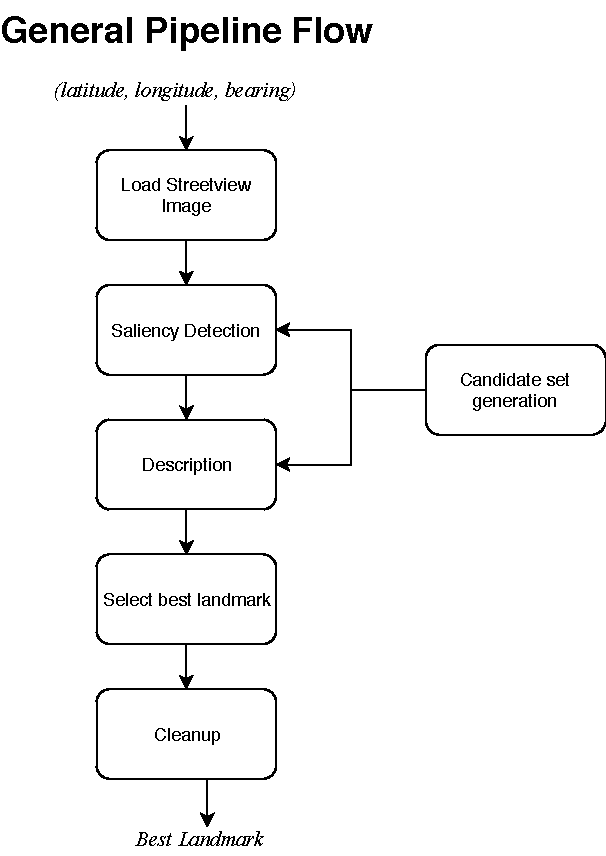
\includegraphics[width=0.6\textwidth]{pipeline_diagrams/general.pdf}
  \caption{The general structure of a Torchbearer pipeline.}
  \label{fig:pipeline:overview}
\end{figure}

While the exact manner in which a pipeline solves the landmark description problem varies from pipeline to pipeline, all pipelines share a general sequence of execution, and all take a tuple consisting of latitude, longitude and bearing as input and yield a tuple containing the best, most salient selected landmark as output.

The first step in any pipeline is to obtain a street-level image of the maneuver point at the given geographic coordinate and bearing. No matter the exact approach the pipeline takes to obtaining a landmark description, it will need this image to perform many of its calculations. Next, the pipeline must generate a set of candidate landmarks, $C$. A candidate landmark is simply an object at the maneuver point that could be used as the basis for a landmark-based instruction. At this point we know nothing about how good a landmark it is, however. 
	
Generation of the candidate landmark set is performed in-band by either the saliency or description step, depending on the pipeline. In pipelines which leverage human-based saliency scoring, the saliency task simultaneously generates a set of candidate landmarks and finds scores for each. Pipelines which use machine-based landmark description will generate a candidate landmark set as part of that step; pipelines which leverage human-based description will rely on the saliency step (whether human or machine-based) to generate a candidate set. 

After the saliency of each candidate landmark has been determined, and each candidate has received a lexical description, the pipeline must decide which landmark is best (most salient). The formula varies by pipeline, and depends on which components of saliency were measured.

\subsection{Saliency}
The saliency portion of a pipeline is responsible for quantifying the saliency of candidate landmarks. While saliency consists of three components--visual, semantic and structural, not all three components are considered individually in each pipeline. Human-based saliency is based on only a single overall score, generated by human opinion, that represents humans' ability to distinguish good landmarks. Machine-based pipelines consider both semantic and visual saliency. In all pipelines, structural saliency is \textit{enforced} rather than \textit{evaluated}: in accordance with the literature, we consider only candidate landmarks that are located at or very near to the maneuver point.

\subsubsection{The Human Approach}
Humans are accustomed to picking out landmarks from their surroundings in day-to-day life, be it for the purpose of giving a friend directions or for their own internalization of a route or location. We can take advantage of this innate ability by asking a human MTurk worker to select what they believe is the most salient, most standout landmark at a given maneuver point. Unlike algorithmic saliency detection, here we do not separate the concept of saliency into its visual and semantic subparts. Rather, we hypothesize that because human workers have an elemental understanding of what makes a landmark salient, the decisions they make regarding the best landmark at a given point will implicitly incorporate these saliency concepts.

Human input is gathered via an MTurk HIT. We denote this type of HIT a Saliency HIT. The Saliency HIT consists of the following task: after the worker elects to work on the task, he is shown a high-resolution image of the maneuver point in question from three distances (at, just before, and before the point.) Note that all three of these images are of equal dimensions. He is asked to use his mouse to draw a bounding box tightly around the object which he believes is the best landmark--the one he would use if he were telling a driver to perform the given maneuver right at that point. He can choose an object in any of the three images, but can only select one object.

Three images from three distances are used so that landmarks of different scales can be captured: a stop sign, for example, is hard to detect in an image from far away, but is prevalent in an image from right near the maneuver point. Likewise, a large building may be an excellent landmark, but might only be visible from some distance away from the maneuver point. In essence, we are showing the worker the approach to, or the path leading up to, the landmark, and allowing them to see what the driver would see at three points along this path. In the final instruction spoken to the driver, the position of the best landmark is taken into account--that is, if the best landmark is one which was selected from the “just before” image, the spoken instruction will tell the driver to turn “just after” the specified landmark.

After the worker makes the worker makes his selection, the coordinates of the drawn bounding box, along with the position corresponding to the image the box was drawn in, are submitted to MTurk. After five workers complete the task, the set of five bounding boxes is sent back to Turk Service. Torchbearer must now aggregate these answers: this particular human task leverages the “sampling and aggregation” approach to human input described in a previous section. That is, because bounding box coordinates are quantitative, we can combine them together in a manner which rewards the “agreement” among workers, if there is any, and culls answers which are in the severe minority and are likely to be meaningless. 

Aggregation is performed by creating a matrix called a \textit{saliency map} for each of three maneuver point images; this matrix represents the number of workers who included each pixel in the bounding box they drew. The creation of this matrix is performed by \ref{alg:saliencyMap}. The result of this operation is a matrix of size equal to the maneuver point images shown to the worker, where an element corresponds to a pixel in the original maneuver point image and where the value of each element is an integer between 0 and $n$, where $n$ is equal to the number of workers. While the saliency map does not incorporate any decision about which regions are or are not salient landmarks, it encodes the relative saliency of each pixel in the image. To make this matrix easier to work with in subsequent pipeline steps, we normalize all values between 0 and 255, where a value of 255 would indicate maximal saliency. A subsequent task in a pipeline can use this saliency map to either find the most salient regions or to query the total saliency of a target region.

\begin{algorithm}[htbp]
%\textbf{Algorithm} Compete
\textbf{Input}: $B$, a set of tuples $(x_1, y_1, x_2, y_2)$ representing bounding boxes;
$m$, the width of maneuver point image;
$n$, the height of maneuver point image; \\
\textbf{Output}: $S$, a matrix of dimension $m$ by $n$ 
\begin{algorithmic}[1]
\State $S\gets 0_{m,n}$
\For{$b \in B$}
\State $S[b.y1:b.y2, b.x1:b.x2] += 1$
\EndFor
\Return{$B$}
\end{algorithmic}
\caption{Creating a saliency map from human input}\label{alg:saliencyMap}
\label{alg:saliencyMap}
\end{algorithm} 

\subsubsection{The Machine Approach}
The algorithmic approach to determining salient landmarks consists of separate components for visual and semantic saliency. However, the machine-based saliency step deals only with visual saliency; semantic saliency is provided as part of the machine-based description step.

Visual saliency refers to the perceptive quality of a region of the driver’s view which causes that region to stand out from its neighbors--that is, the degree to which a region grabs a driver’s visual attention. Street-level imagery of a maneuver point serves as input; the goal is to quantify each pixel of a maneuver point image in terms of its relative visual saliency. Specifically, given an $m x n$ input image of a maneuver point, an $m x n$ \textit{saliency map}, is output where each element in the matrix is an integer between 0 and 255 corresponding to how visually salient that pixel is. A value of 0 indicates no saliency, while a value of 255 indicates maximal saliency.

Torchbearer leverages a state-of-the art, deep-learning based algorithm called SalNet \cite{Pan_2016_CVPR} to estimate the pixel-level visual saliency across an image. Rather than seeking to identify specific neuroscience-inspired image features which identify saliency, as many previous approaches do, SalNet takes a completely data-driven approach, using a deep convolutional neural network to “learn” where the human gaze tends to fixate in different images. Training data consists of a large dataset of ImageNet \cite{imagenet_cvpr09} images, each with a corresponding ground truth \textit{saliency map}. This dataset was created by tracking subjects’ gaze as they were shown each image and recording the time gaze was focused on each pixel. These gaze times were then normalized to between 0 and 255, inclusive.

SalNet uses a deep neural network architecture to predict the saliency map for an input image. The first three layers of this network consist of pretrained layers from a Visual Geometry Group image classification network, VGG16 \cite{Simonyan14c}; the authors recognize that the low-level features learned by these layers offer valuable input to the saliency problem. VGG16 has been trained on an extremely large dataset, and by using transfer learning, SalNet can benefit from this extensive training without needing to train on so many images itself. The pretrained network is followed by a series of convolutional and pooling layers and finally a deconvolutional layer, which will cast the output back into a matrix of the same size as the input. Training of the neural network consists of minimizing the Euclidean distance between the saliency map output by the network and the ground truth saliency map provided by the training dataset. During training the weights of the first three layers are fixed at the pretrained weights from the VGG16 network; only the additional, saliency-specific layers unique to SalNet are actively trained.

It is important to note that SalNet is trained on a wide range of ImageNet images from across a broad range of topics; it does not incorporate any knowledge specific to the navigation domain. At the time of writing, no dataset containing ground truth saliency maps for street-level imagery was available of sufficient size for training a neural network. Training the SalNet architecture with domain-specific data would certainly be worthwhile future work. However, the general principles of visual saliency are not specific to any single domain, and the generalized training of SalNet allows it to perform well on an evaluation set of images from across the ImageNet corpora. We have hypothesized that it can adequately generalize to the navigation domain.

\begin{figure}[htbp]
  \centering
  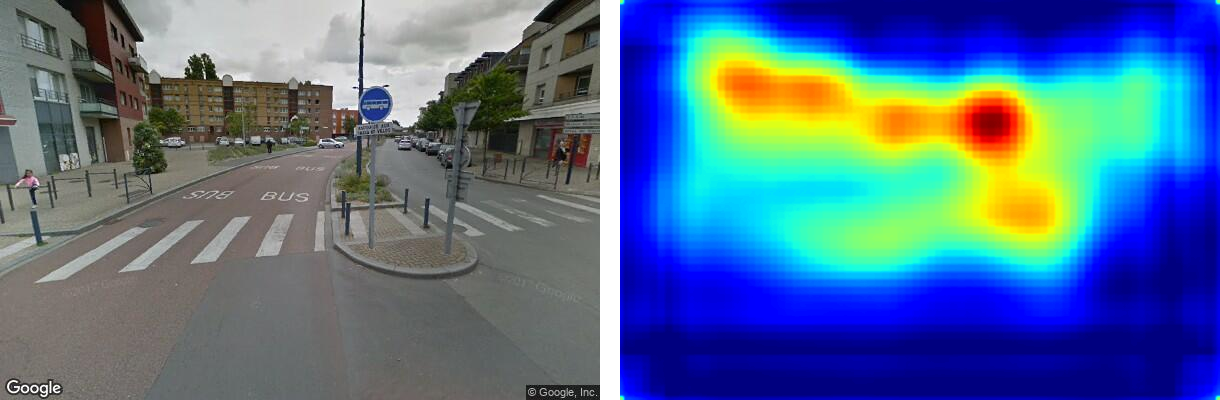
\includegraphics[width=0.6\textwidth]{images/saliencyMap.png}
  \caption{Left: a maneuver point image. Right: a corresponding saliency map generated by SalNet}
  \label{fig:saliencyMap}
\end{figure}

\subsection{Description}
The second half of the landmark selection problem consists of deriving a lexical description of a candidate landmark, although the machine approach to description is also responsible for generating candidate landmarks as well as providing semantic saliency scores. This description should be specific enough so as to allow a driver to easily distinguish that given landmark from its surroundings.

\subsubsection{The Machine Approach}
Torchbearer leverages two approaches for finding semantically salient landmarks and quantifying their salience: a data driven approach, which uses a geosocial datasource to estimate the local significance of business and points of interest, and a deep learning-based object detection algorithm which searches for known semantically salient features in maneuver point images.
	
\subsubsubsection{Data-driven Approach}
Torchbearer estimates the semantic saliency of a landmark via an estimate of the number of people who have recently visited the landmark, as counted by the social networking application FourSquare. Previous work has shown the efficacy of using geosocial streams as a proxy for the local importance of a landmark; the intuition being that the more people who have “checked in” to a given location, the more well-known, or prominent, it is \cite{quesnot2014measure}. FourSquare incorporates businesses, points of interest and publicly accessible places into its ecosystem; these are known as venues. User location is recorded transparently, without the need for them to explicitly tap a "check in" button Torchbearer leverages FourSquare’s venue data both to find candidate landmarks and determine their semantic saliency. 

To find candidate landmarks for a given maneuver point, Torchbearer queries FourSquare for venues which are within a given radius of the maneuver point. By default, a small 100-foot radius is used, in the aim of ensuring any returned venue will be on or near the road upon which the maneuver point is located. FourSquare returns a list of tuples consisting of the venue name, the type of venue (such as restaurant, gas station, etc.) the geographic coordinates and the number of FourSquare users who have “checked in” to that venue. 

We compute the relative bearing between the venue and the approach bearing of the user, and discard venues which are not within 45-degrees of either side of the user, as the field-of-view of our street-level imagery is 90-degrees.
Each of these venues is converted to a Landmark: the landmark's description is the name of the FourSquare venue, concatenated with its category. For example, the description for a landmark corresponding to a venue with the name “Starbucks” and category “Coffee Shop” would be “Starbucks Coffee Shop”. The landmark’s semantic saliency score $S_s$ is function of the number of checkins in the last six months $c$ and the number of locations $l$, if the venue is a chain:

\begin{equation}
    S_s = c + l
\end{equation}

This measure captures both the local significance and wide-area ubiquity of the landmark.

\subsubsubsection{Object detection approach}
Some landmarks are ubiquitous and proven to be highly semantically salient, independent of the maneuver point's geographic location. Road infrastructure, such as stop signs and traffic lights, is a prime example: these landmarks are universally recognizable among drivers, and have been shown to serve as excellent landmarks for use in navigation instructions \cite{may_ross_bayer_2005}. Unfortunately, we found no dataset of street signage or traffic lights with coverage beyond a specific locality. Instead, we leverage a state-of-the-art object detection algorithm, Faster-RCNN, to detect stop signs and traffic lights at maneuver points. Note that as a direction for future research, extending the object detection model to include other types of landmarks is both feasible and potentially beneficial.

Faster-RCNN (FRCNN) \cite{ren2015faster} is a deep, region-based, convolutional neural network which takes an image as input and yields a set of bounding boxes, class labels (a string denoting which object the region was classified as) and confidence scores for objects of interest detected within the image. It is currently one of the highest performing classifiers in terms of both speed and accuracy, 

FRCNN leverages an existing image classification network, ResNet, to compute feature maps for an image, and then uses the output of an intermediate convolutional layer in that "base" network as input to its own FRCNN-specific layers. This is known as transfer learning, and allows an FRCNN model to take advantage of the extensive training across millions of ImageNet images encoded within ResNet. The output of this intermediate convolutional layer, although trained on ImageNet data, outputs high-level image features as opposed to specific classes probabilities. Using these high-level feature maps as input, FRCNN will train its own final (fully-connected) layers to output class probabilities specific to our data.

FRCNN consists of two sub-networks: a Region Proposal Network (RPN) which is trained to output a set of possible bounding boxes, and the CNN network itself, which performs classification and final bounding box adjustment (based on the predicted class). To predict likely bounding boxes, the RPN considers all possible \textbf{anchor boxes}. An anchor box is simply a fixed set of 9 on candidate bounding boxes of different sizes and aspect ratios anchored at every point in the image. For example, if the input image is of dimensions $n x n$, then there will be $9n^2$ anchor boxes for the RPN to consider. For each anchor box, the RPN learns to output (through the use of three convolutional layers) a probability corresponding to likelihood of the box containing an object of interest, as well as a tuple of four doubles indicating the amount by which to adjust each coordinate of the predefined anchor box. Boxes with a probability of objectiveness below  certain threshold are discarded, the rest are passed on to the classification sub-network.

Given a set of possible bounding boxes generated by the RPN, the CNN first uses Region of Interest Pooling (ROI) to generate fixed-size convolutional feature maps corresponding to the region of the input feature map contained within each bounding box. ROI consists of splitting the box into $k$ evenly sized regions and selecting the maximal value from each region, yielding a feature map of size $k$, where $k$ is a small integer, often 7. This pooled feature map is then input to two successive 4096-neuron fully-connected layers--these two layers learn the actual classification function. 

The output of the second fully-connected layer is passed through a softmax layer of size equal to $c + 1$, where $c$ is the number of classes we are trying to predict. (The extra output is for the "background" class--a bounding box that did not contain an object.)  The softmax layer gives a floating-point number for each output, subject to the following constraint: let $Y$ be the set of outputs, then 
\begin{equation}
    \sum\limits_{y \in Y} y = 1
\end{equation}

This gives a probability distribution over the set of possible classes for the likelihood of an object being a particular class (or background).

In addition to the softmax output corresponding to class predictions, the network outputs a tuple of bounding box adjustments corresponding to each class. (These are output via a single fully-connected layer of size $4c$.) For each prediction rendered by the network, 

We constructed a dataset of 800 street-level images and ground-truth bounding boxes. Each image contained traffic lights, stopsigns or both. We generated an addition 75 negative examples--images containing neither a stoplight nor a stop sign. This dataset was divided into training and test sets, with a split of 85\% train and 15\% test. We trained an FRCNN network for 20 epochs--that is, 20 complete passes through our training set. At the completion of training, we achieved a mean average precision on our test dataset of 0.71 for stop lights and 0.75 for stop signs.
	
\subsubsection{The Human Approach}
To gather human descriptions for a given landmark, we again leverage Mechanical Turk. However, instead of using a sampling approach as we did with saliency crowdsourcing, we use a verification approach.
First, for a candidate landmark $c$, the street-level image of the maneuver point for which this landmark is a candidate is annotated to include a bounding box drawn around the landmark. An MTurk HIT is created with only a single assignment; the worker will be shown this image and asked to describe the enclosed object. The exact format of the question is: \texit{“Provide a specific description of the main object in the box. Describe PERMANENT, man-made things--NOT cars, people or things that could move.  Pretend you were using that object as a landmark when giving someone directions.”} The worker is given a text box into which to type their answer.

After the worker has submitted the description, a verification HIT is created on MTurk, with three assignments. Each worker will be shown the annotated maneuver point image along with the candidate description and asked to decide whether the description is accurate and meets the criteria of describing “permanent, man-made things--not cars, people or things that could move”. (Two radio buttons are displayed—”yes” and “no”.)

 If at least two of the three workers indicate that the description is accurate, the description is accepted, and pipeline execution can continue. If not, the process repeats, with the creation of a new description HIT and subsequent verification HITs. Torchbearer will retry this process up to three times--if no description could be derived, the landmark is removed from the candidate set and pipeline execution continues.

\subsection{Finding landmarks in saliency maps}
Given a saliency map, it is often important to locate candidate landmarks based on “hot spots”, or highly salient regions, in the map. The significance of this is different for human-based saliency detection than for machine-based saliency detection.

With human-based saliency detection, the goal is to reduce the set of returned bounding boxes into a reduced set of distinct landmarks by combining overlapping bounding boxes into a single area. For example, of the five answers it might be that three bounding boxes mostly overlap, indicating that that those workers intended to select the same landmark, while the other two answers overlap a separate landmark. Rather than treat all five bounding boxes as separate landmarks, it is beneficial to instead consider only the two distinct landmarks. First, this reduces the scale of future pipeline operations--they do not need to perform (redundant) calculations on as many candidate landmarks. This saves time and compute cycles and, in the case of human-based tasks, fees paid to workers. Second, by reducing bounding boxes into single areas we can assign a saliency score to the candidate landmark based on how many answers included it in their bounding box. This can be used at the end of the pipeline as part of the decision process for choosing the best landmark. It is this score that acts as proxy for human intuition into what makes the best landmark: the more workers who select a landmark, the better it should be.

In the case of machine-based saliency, it is necessary to correlate the set of candidate landmarks generated by the semantic saliency (FourSquare-based) step with an area of the visual saliency map. While we know the latitude and longitude of the candidate landmark, we do not directly know the area it occupies in the saliency map. In order to find the visual saliency of that candidate landmark we must estimate its location in the saliency map. This requires us to locate potential salient regions in the saliency map, so that we can determine if the candidate landmark aligns with one of those regions. 
Given a saliency map, a matrix of values ranging from 0 to 255, the goal is to label each pixel as belonging to a specific salient region or being non-salient. 

Non-maximal suppression (NMS) is a state-of-the-art method for reducing a set of bounding boxes to only the significant ones, discarding bounding boxes which enclose the same region using greedy clustering and a fixed distance threshold \cite{neubeck2006efficient}. If our saliency map were composed of entirely rectangular regions of different saliency values (as is actually the case with human-based saliency detection) this method would be sufficient. However, the saliency map returned by our computer-vision based saliency algorithm estimates saliency at the pixel level and, as a result, makes no guarantee about the shape of salient regions.

The Watershed Algorithm is an image segmentation approach, designed to single out distinct regions in the image by separating foreground elements from background elements \cite{barnes2014priority}. In classic image processing, these regions might be objects one wishes to separate from on In our case we wish to separate regions of relatively high saliency (foreground) from their low-saliency surroundings (background). The algorithm works by considering our saliency map as a topological surface, where the value of a pixel denotes its height--pixels with a value of 0 (no saliency) are valleys and pixels with a value of 255 (highest saliency) are peaks. For each valley, or minima, in the map, the algorithm fills the topology with different-colored water--that is, it labels pixels as belonging to a given segment. As the water level rises, water from different valleys will begin to converge. To prevent this, the algorithm constructs infinitely tall barriers, or segmentation lines, between the two valleys. This process is continued until even the tallest peak is submerged, leaving only the barriers above water. These barriers now encapsulate different objects, or salient regions, within the map. 

To make this algorithm more impervious to over-segmentation and noise--small regions of high salience within a low-salience area or vise versa--we leverage the marker-controlled watershed algorithm \cite{roerdink2000watershed}. Here, we dictate to the algorithm which pixels we know to be independent, salient regions, which ones we know to be non-salient, background pixels and which ones we are unsure about, the border area between known salient regions and non-salient background. Now, rather than flooding starting at the minima, the algorithm begins flooding from each foreground region and the background region; it is now simply finding where the segmentation line will be placed within the unknown border area.

In order to apply the watershed algorithm, several preprocessing morphological steps must be taken to “clean up” the saliency map, and each pixel must be labeled according to its status as known background, known foreground, or unknown. The following steps outline this process, given a saliency map $S$:

\begin{enumerate}
\item
Perform binary segmentation on $S$, rendering each pixel as salient (255) or non-salient (0). (This renders a “black and white” image.) This is completed by finding a threshold $t$, at or above which a pixel is considered salient and below which a pixel is considered non-salient. $t$ is selected via Otsu Thresholding \cite{otsu1979threshold}, which works by iterating through all possible threshold values and selecting the one which minimizes the sum of the weighted variances within the salient and non-salient classes. That is,

\begin{equation}\label{eq:otsu}
    threshold=argmin_t(\frac{\mid n \mid}{\mid n \mid +\mid s \mid} \sigma_{n}^{t} + \frac{\mid s \mid}{\mid n \mid + \mid s \mid}\sigma_{n}^{t})
\end{equation}

Where $t$ is the candidate threshold, $s$ is the set of salient pixels, $n$ is the set of non-salient pixels and $\sigma$ is the variance within the given set of pixels when a given $t$ is used as the threshold value.

\item
Remove small, insignificant salient areas (white noise) by performing morphological opening on the binary segmentation.

\item
Remove small, insignificant non-salient areas (holes) by performing morphological closing on the binary segmentation.

\item
Determine which pixels are known to be non-salient by dilating the binary segmentation, falsely enlarging the salient regions. Dilation consists of scanning a square kernel $K$ over the binary segmentation and, at each point, replacing the binary segmentation pixel underneath the anchor point (center) of $K$ with the maximal value overlapped by $K$. Denote this dilation as $M_n$.

\item
Apply a distance transformation to the binary segmentation, resulting in the value of each pixel being equal to the Euclidean distance between that pixel and a pixel with value 0 (non-salient background). This is essentially finding salient peaks, or the centers of salient regions, as the pixels which are farthest from a non-salient pixel are the ones in the center of a large salient region. Denote this distance transform as $D$.

\item
Determine pixels which are known to be salient by applying a binary threshold to the distance transform, where $t$, the threshold, is set to $c * max(D)$ where $c$ is a constant factor which we set to 0.7. The goal is to isolate salient pixels which are far from any non-salient pixels, as we can be confident that these are salient pixels. Denote this threshold $M_s$.

\item
Pixels which are not known to be either salient or non-salient are found by $M_u = M_s - M_n$.

\item
Each distinct (disconnected) region of salient pixels in $M_s$ needs to be labeled from $2...n+1$, where $n$ is the number of distinct regions. The background, or non-salient-pixels, must be labeled as 1. This is accomplished by performing a connected component analysis on $M_s$ with 8-connectivity, yielding $M_m$, a matrix with consecutively labeled connected components. 
Label the unknown region with 0; this is the region in which watershed will draw a segmentation line to determine the final boundary around the salient regions. Specifically, $\forall p_{ij} \in M_u \mid p=0, M_l[i, j] = 0$

\item
Run the watershed algorithm on $S$, using $M_l$ as markers. The returned matrix $M_w$ will have labeled all pixels as non-salient (1) or as belonging to a salient region (2...n+1).

\item
The final step is to calculate the bounding box around each salient region in $M_w$; these are our landmarks.
\end{enumerate}

\subsection{Quantifying Landmark Uniqueness}\label{sec:unique}

The semantic uniqueness of a landmark is an important factor in its saliency \cite{caduff2008assessment}. Even for pipelines that leverage human-based saliency detection, and thus don not componentize the saliency score, uniqueness is still used for tie breaking purposes.

We use the lexical description of a landmark to derive its uniqueness as compared to the rest of the candidate landmark set. Our approach is based on word embeddings, where a word is represented as a high-dimensional vector in vector space \cite{goldberg2014word2vec}. The value in such a framework stems from the Distributional Hypothesis, which contends that words which are semantically similar will be distributionally similar as well, appearing together in the same contexts \cite{harris1954distributional}. The goal in creating vectorizations of a set of words is to represent semantically similar words with similar as, i.e. close, points in high-dimensional space. This allows us to determine the similarity of words by comparing the Euclidean distance between the points or cosine similarity between the corresponding (normalized) vectors.

\subsubsection{Word2Vec}
A common method for generating the vector representations of a set of words is to use a predictive model, where a machine learning algorithm learns to accurately predict a word's context, or words that are likely to appear around it, given only the word \cite{baroni2014don}. One such model, Word2Vec, \cite{mikolov2013efficient} is trained to predict a nearby word given another word, effectively internalizing a representation of which words appear in the same contexts. The algorithm uses a neural network with a hidden layer os size equal to the desired dimensionality of the word embedding.  Using a large corpus of text, and a selected vocabulary of important words therein, the network is trained to accurately predict the probability of each word in the vocabulary occurring within a small window of an input word in the corpus. In doing so, the algorithm generates a $v x d$ weight matrix (from the hidden layer to the output layer) which acts as a function from $word : P$, where $v$ is the size of the vocabulary, $d$ is the dimensionality of embeddings and $P$ is a vector of probabilities for each word in the vocabulary. After training, each row in this matrix represents the embedding for a word in the vocabulary. Intuitively, if two words are similar, they are likely to be surrounded by similar words, per the Distribution Hypothesis. Thus, they will have learned similar weights, so as to generate similar probability distributions over the vocabulary.

We use a pretrained word2vec model \cite{word2vec} with 300-dimensional word embeddings, trained on the Google News corpus and containing 300 million vocabulary words. We use cosine similarity as a measure of similarity between word embeddings, meaning that our similarity measure is bound between [-1, 1], with 1 indicating complete similarity and -1 indicting complete lack of similarity. 

To find the similarity between two landmark description phrases, we compute a description vector which is a sum of the vectors of each word in the description and then calculate the similarity between those two vectors. Given two candidate landmarks $c_1$ and $c_2$, the similarity $s$ between these landmarks is defined as

\begin{equation}\label{eq:landmrkSimilarity}
    pairSimilarity = (c_1, c_2) \longrightarrow c(\sum\limits_{w \in c_1.description} embedding(w), \sum\limits_{w \in c_2.description} embedding(w))
\end{equation}

where $embedding$ is the word2vec vector for the given word and $c$ is the cosine similarity function of two vectors $v_1$ and $v_2$:

\begin{align}\label{eq:cosineSimilarity}
    c &= (v_1, v_2) \longrightarrow cos(\theta)
      &= (v_1, v_2) \longrightarrow \frac{A \cdot B}{\parallel A \parallel \parallel B \parallel}
\end{align}

where $\theta$ is the angle between the two vectors.

To find the similarity of a landmark $c$ as compared to all other landmarks in a set of candidate landmarks $C$:

\begin{equation}\label{eq:landmrkSimilarityOverall}
    totalSimilarity = \sum\limits_{k \in C} pairSimilarity(k, c)
\end{eqaution}

\section{Pipeline Specifics}
\subsection{Machine-Machine}

\textbf{Input}: $I_0 = (latitude, longitude, bearing)$
\textbf{Output}: The most salient landmark, including a description for use in navigation instructions
\textbf{Candidate selection}: Description

\begin{figure}[htbp]
  \centering
  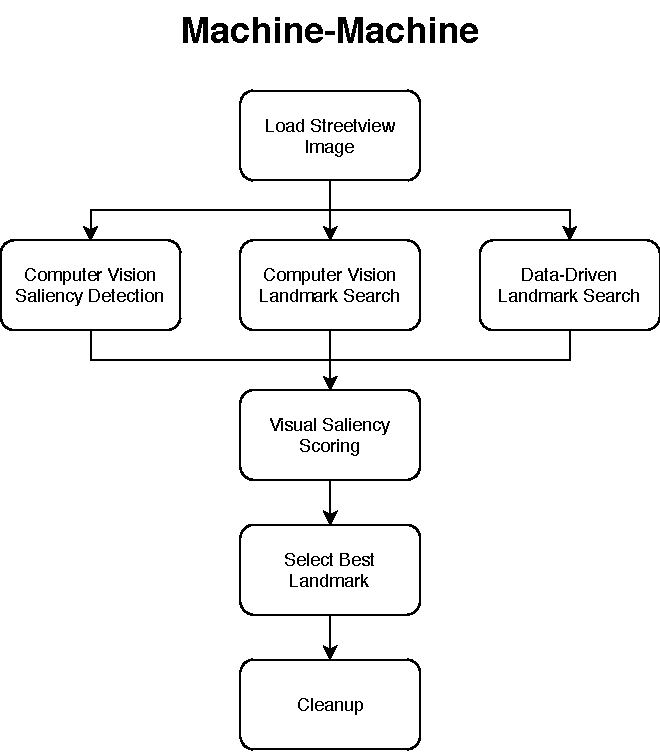
\includegraphics[width=0.6\textwidth]{pipeline_diagrams/machine-machine.pdf}
  \caption{The pipeline structure of the Machine-Machine pipeline.}
  \label{fig:pipeline:mm}
\end{figure}

\subsubsection*{Step 1: Load Streetview Image}
\textbf{Input}: $X_0 = (latitude, longitude, bearing)$
\textbf{Output}: $Y_0 = (latitude, longitude, bearing, [image_urls])$

This step consists of querying the Google Streetview API for street-level imagery at distances of 25, 50 and 100 feet from the given coordinate at an angle opposite of the bearing. (We refer to these distances relatively as “at”, “just before” and “before”.) Returned images are stored on Amazon Simple Storage Service (S3), and the S3 URL of each image is added to a tuple which is included in the output of this step. 

\subsubsection*{Step 2a: Computer Vision Saliency Detection}
\textbf{Input}: $X_{2a} = Y_0 = (latitude, longitude, bearing, [image_urls])$
\textbf{Output}: $Y_{2a} = (latitude, longitude, bearing, [image_urls], [saliency_matrices])$ 

Implementing the machine approach methodology outlined in the Saliency section, this step uses the SalNet deep learning architecture to compute a saliency map for each image in the tuple of images in $X_{2a}$. The processing of each image happens in parallel, and consists of feeding the the street-level image through SalNet and capturing the output.

For each image, this step yields a one-dimensional matrix of the same shape as the input image, with values ranging between 0 and 255, inclusive. Each matrix is included in the output tuple provided to subsequent pipeline steps.

\subsubsection*{Step 2b: Computer Vision Landmark Search}
\textbf{Input}: $X_{2b} = Y_0 = (latitude, longitude, bearing, [image_urls])$
\textbf{Output}: $Y_{2b} = (latitude, longitude, bearing,  [image_urls], [candidate_landmarks] )$ 

This step uses the Faster RCNN-based object recognition algorithm, described in the Saliency section, to detect candidate landmarks in each maneuver point image. The network has been trained to detect stop signs and stop lights; it returns, for each object it detects, a tuple consisting of the coordinates of the object’s bounding box within the image, a confidence score between 0 and 1 and a description (label) for the object. We discard any objects with a confidence score less than 0.8 based on the notion that it is better from a usability standpoint to not provide a landmark description in an instruction than it is to provide a description of a nonexistent landmark. The remaining objects are converted into candidate landmark tuples, with a semantic saliency score of 1.0. (We assume that all users are fully aware of what a stop sign or stoplight looks like, thus no other landmark can be more semantically salient than a landmark detected by this step.) These landmarks are included in the output of this step.

\subsubsection*{Step 2c: Data-driven Landmark Search}
\textbf{Input}: $X_{2c} = Y_0 = (latitude, longitude, bearing, [image_urls])$
\textbf{Output}: $Y_{2c} = (latitude, longitude, bearing,  [image_urls], [candidate_landmarks], [saliency_matrices] )$ 

This step uses FourSquare to find candidate landmarks by searching for venues within a 50-foot radius of the maneuver point, as detailed in the Saliency section. Candidate landmarks are included in the output tuple.

\subsubsection*{Step 3: Visual Saliency Scoring}

\textbf{Input}: $X_3 = Y_{2a} \cup Y_{2b} \cup Y_{2c} = (latitude, longitude, bearing,  [image_urls], [saliency_maps], [candidate_landmarks] )$
\textbf{Output}: $Y_3 = (latitude, longitude, bearing,  [image_urls], [candidate_landmarks] )$ 

This step assigns a quantitative score to each candidate landmark designating its visual saliency in the context of the maneuver point image. The computer-vision based saliency detection approach is not landmark-aware; that is, it determines relative saliency at the pixel-level. This step aggregates these pixel-level values into a score for the entire landmark. Given the bounding box coordinates $x_1, x_2, y_1,y_2$ of a candidate landmark and the saliency map $S$ of the maneuver point, the visual saliency score of that candidate is calculated as

\begin{equation}
    score= \frac{\sum\limits_{i=x_1}^{x_2} \sum\limits_{j=y_1}^{y_2} S_{ij}}{\sum S}
\end{equation}

That is, the visual saliency score is the sum of the submatrix contained within the bounding box divided by the sum of the entire saliency map. This gives two desirable properties: first, the larger a landmark is, the higher its score. Second, the more high-saliency pixels contained within a landmark bounding box, the higher its score.

While candidate landmarks detected by the object detection and human-based approaches include bounding boxes, and can therefore be correlated directly with a region in the saliency map, those returned by the data-driven approach do not. For these candidates, only the relative bearing between the maneuver point and landmark is known. In order to estimate which rectangular region of the saliency map corresponds to these landmarks we must first locate salient regions within the saliency map and then determine if one of those regions lies on the given bearing.

To locate salient regions, we use the watershed-based approach described previously. This lends us a set of bounding boxes, each containing a salient region within the saliency map. To determine if one of these salient regions represents our candidate landmark, we consider two points facts about the street-level image off of which the saliency map was created: first, the pitch of the image is zero degrees, meaning that the horizon line, where a venue would be, is roughly in the vertical middle of the image. Second, the field of view of the image is 90-degrees, and is not distorted or warped. Given the relative bearing between the maneuver point and the landmark, we check if there exists a salient region at this bearing in the vertical middle of the saliency map. (See Figure X.) If there is, we use this region as the bounding box for the candidate, and calculate the visual saliency score as above. If not, we assign a score of 0, as we have no evidence as to the visual saliency of this landmark.

\begin{figure}[htbp]
  \centering
  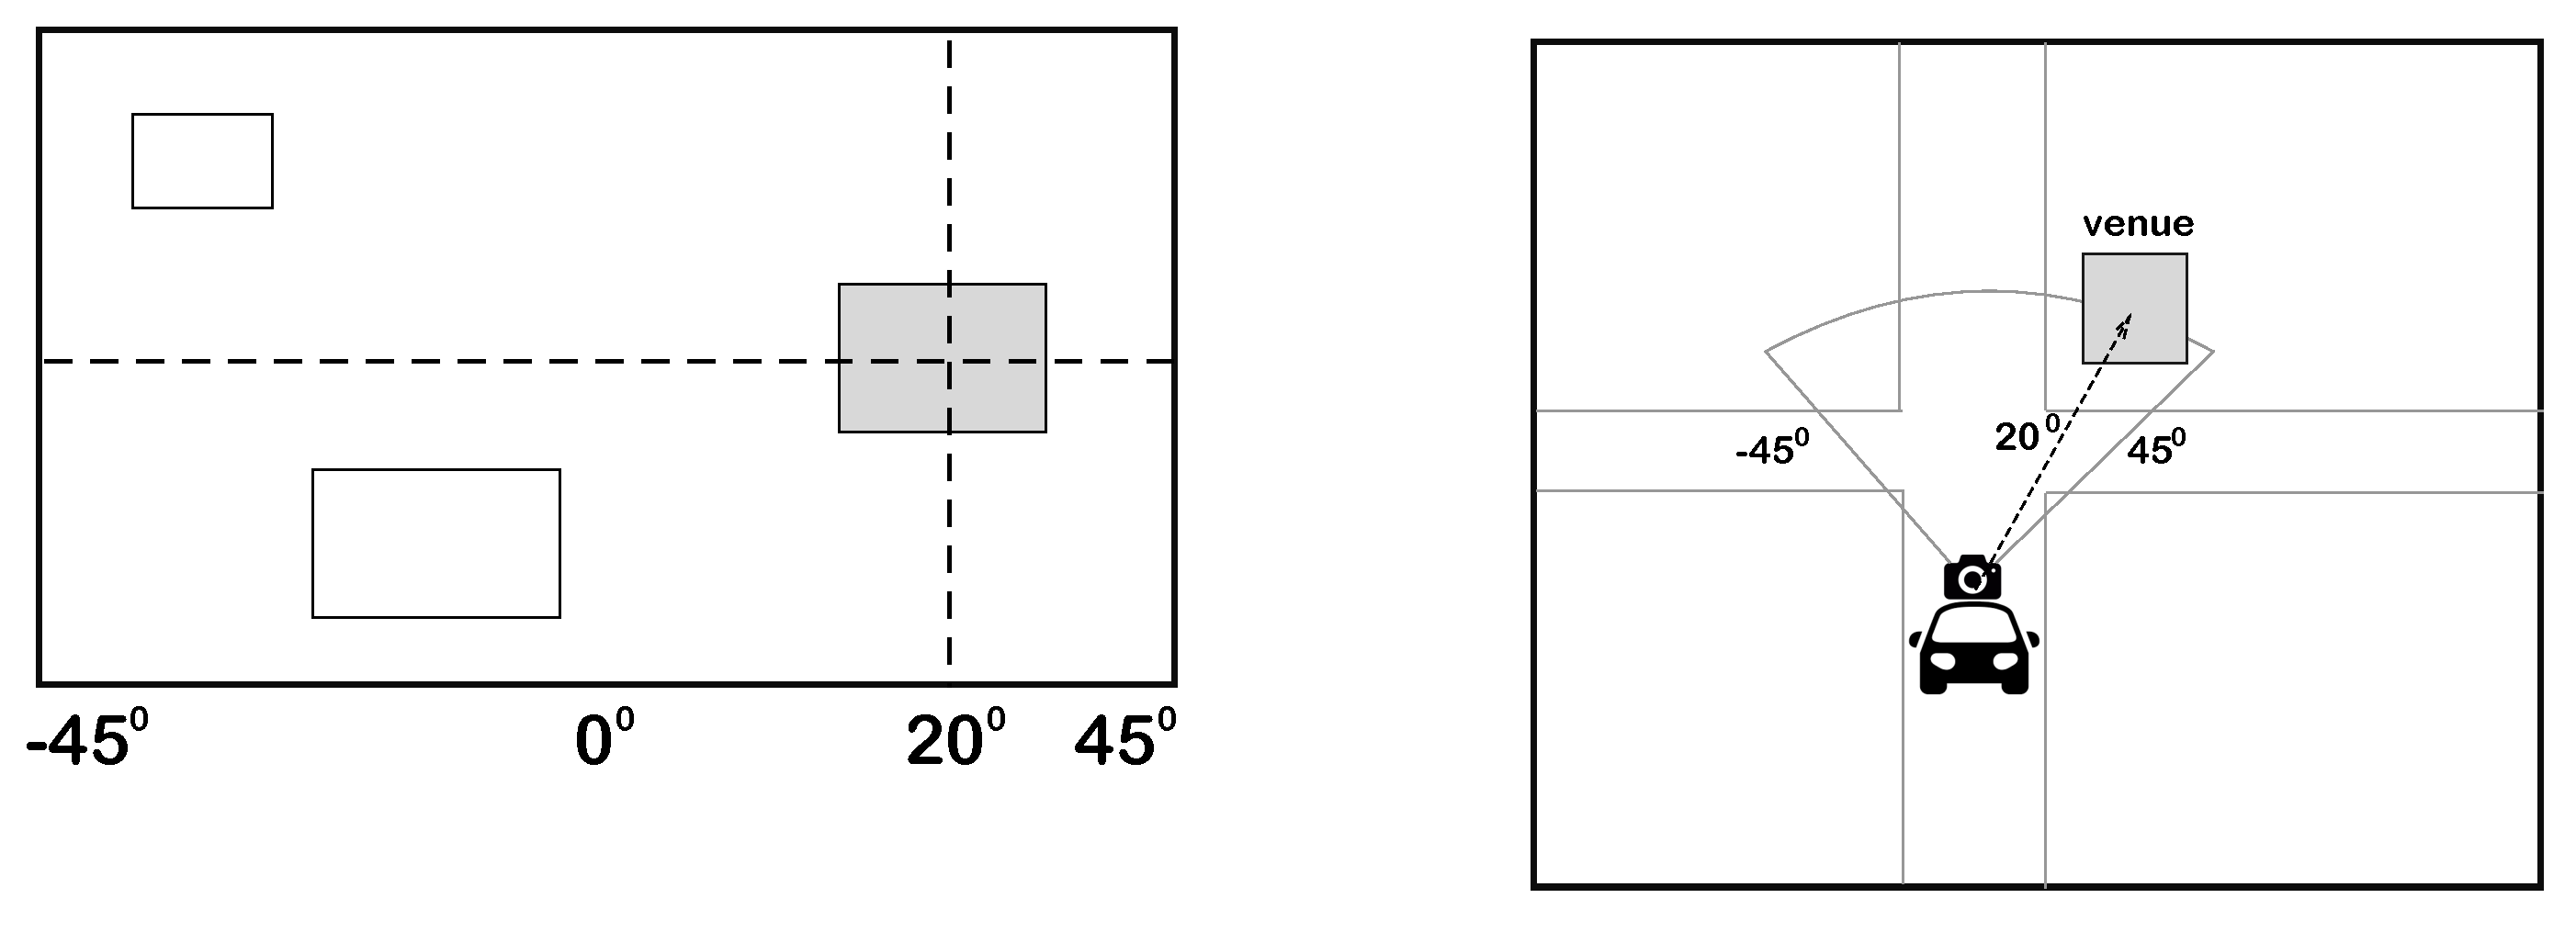
\includegraphics[width=0.6\textwidth]{images/landmark_search.pdf}
  \caption{Left: a landmark saliency map, with bounding boxes of salient regions. The intersection between the relative bearing parallel and vertical middle is within a salient region. Right: A bird's eye view of an intersection. Our street-level images are a rectilinear projection of a spherical image covering a 90 degree field of view.}
  \label{fig:pipeline:mm}
\end{figure}

\subsubsection*{Step 4: Select Most Salient Landmark}

\textbf{Input}: $X_4 = Y_3 = (latitude, longitude, bearing,  [image_urls], [saliency_maps], [candidate_landmarks] )$
\textbf{Output}: $Y_4 = (latitude, longitude, bearing, best_landmark)$ 

At this point in the pipeline, we have a set of candidate landmarks, each complete with both a visual and semantic saliency score. In order to determine the best, most salient landmark, we must first determine the uniqueness saliency score for each candidate, calculated via the method described in \ref{sec:unique}. Next, we normalize each of the three saliency scores to a value between 0 and 1. Given a set of candidate landmarks $C$, the normalized score for a given saliency component (visual, semantic or structural) for a given landmark $c$ can be found by

\begin{equation}
    score_{component} = \frac{c_{score}}{max_{i \in C}(i_{score})}
\end{equation}

The total saliency score for a candidate is then the sum of the three normalized scores. 

\begin{equation}\label{eq:saliency}
    S = S_v + S_s + S_u
\end{equation}

where $S_v$ is the visual saliency score, $S_s$ the semantic saliency score, and $S_u$ the uniqueness score, .

The candidate landmark with the highest summed scores is the best, most salient landmark, and is the output of this step. The description of this landmark will be included in navigation instructions spoken to the user.

\subsubsection*{Step 5: Cleanup}

\textbf{Input}: $X_5 = Y_4 = (latitude, longitude, bearing, best_landmark)$
\textbf{Output}: $Y_5 = (best_landmark)$

This final step consists of system cleanup tasks. All intermediate images stored on S3 are removed--namely, street level imagery. The best landmark is stored in a database, associated with the maneuver point and pipeline identifier for future retrieval.

\subsection{Human-Machine}
\textbf{Input}: $X_0 = (latitude, longitude, bearing)$
\textbf{Output}: The most salient landmark, including a description for use in navigation instructions
\textbf{Candidate selection}: Description

\begin{figure}[htbp]
  \centering
  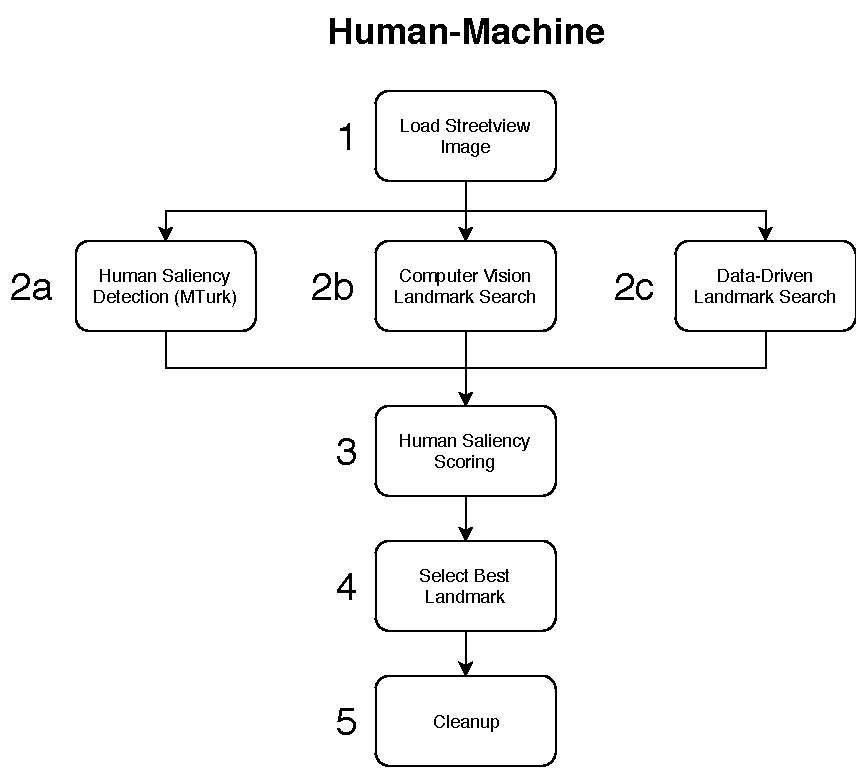
\includegraphics[width=0.6\textwidth]{pipeline_diagrams/human-machine.pdf}
  \caption{The pipeline structure of the Human-Machine pipeline.}
  \label{fig:pipeline:hm}
\end{figure}

\subsubsection*{Step 1: Load Streetview Image}
\textbf{Input}: $X_1 = X_0 = (latitude, longitude, bearing)$
\textbf{Output}: $Y_1 = (latitude, longitude, bearing, [image_urls])$

This step is implemented in the same manner as Step 1 of the Machine-Machine pipeline.

\subsubsection*{Step 2a: Human Saliency Detection} 
\textbf{Input}: $X_{2a} = Y_1 = (latitude, longitude, bearing, [image_urls])$
\textbf{Output}: $Y_{2a} = (latitude, longitude, bearing, [image_urls], [saliency_matrices])$ 

This step generates a saliency matrix for the maneuver point, based off of the street-level image. This implementation uses the crowdsourcing approach described in the Saliency section, and leverages human intuition about what constitutes a good landmark. The saliency map generated is therefore not specific to a single component of landmark saliency (visual, semantic or structural) but comprises the entire saliency metric. 

The output of this step is a matrix of the same dimensions as the input maneuver point image; each element is a value between 0 and 255 indicating the relative saliency at that point in the image.

\subsubsection*{Step 2b: Computer Vision Landmark Search}
\textbf{Input}: $X_{2b} = Y_1 = (latitude, longitude, bearing, [image_urls])$
\textbf{Output}: $Y_{2b} = (latitude, longitude, bearing,  [image_urls], [candidate_landmarks] )$ 

This step is implemented in the same manner as Step 2b of the Machine-Machine pipeline.

\subsubsection*{Step 2c: Data-driven Landmark Search}
\textbf{Input}: $X_{2c} = Y_1 = (latitude, longitude, bearing, [image_urls])$
\textbf{Output}: $Y_{2c} = (latitude, longitude, bearing,  [image_urls], [candidate_landmarks], [saliency_matrices] )$ 

This step is implemented in the same manner as Step 2c of the Machine-Machine pipeline.

\subsubsection*{Step 3: Visual Saliency Scoring}

\textbf{Input}: $X_3 = Y_2 = (latitude, longitude, bearing,  [image_urls], [saliency_maps], [candidate_landmarks] )$
\textbf{Output}: $Y_3 = (latitude, longitude, bearing,  [image_urls], [candidate_landmarks] )$ 

This step is implemented in the same manner as Step 3 of the Machine-Machine pipeline.

\subsubsection*{Step 4: Select Most Salient Landmark}

\textbf{Input}: $X_4 = Y_3 = (latitude, longitude, bearing,  [image_urls], [saliency_maps], [candidate_landmarks] )$
\textbf{Output}: $Y_4 = (latitude, longitude, bearing, best_landmark)$
 
The candidate landmark with the highest human saliency score is the best, most salient landmark, and is the output of this step. The description of this landmark will be included in navigation instructions spoken to the user.

\subsubsection*{Step 5: Cleanup}

\textbf{Input}: $X_5 = Y_4 = (latitude, longitude, bearing, best_landmark)$
\textbf{Output}: $Y_5 = (best_landmark)$
This step is implemented in the same manner as Step 5 of the Machine-Machine pipeline.

\subsection{Machine-Human}
\textbf{Input}: $X_0 = (latitude, longitude, bearing)$
\textbf{Output}: The most salient landmark, including a description for use in navigation instructions
\textbf{Candidate selection}: Saliency

\begin{figure}[htbp]
  \centering
  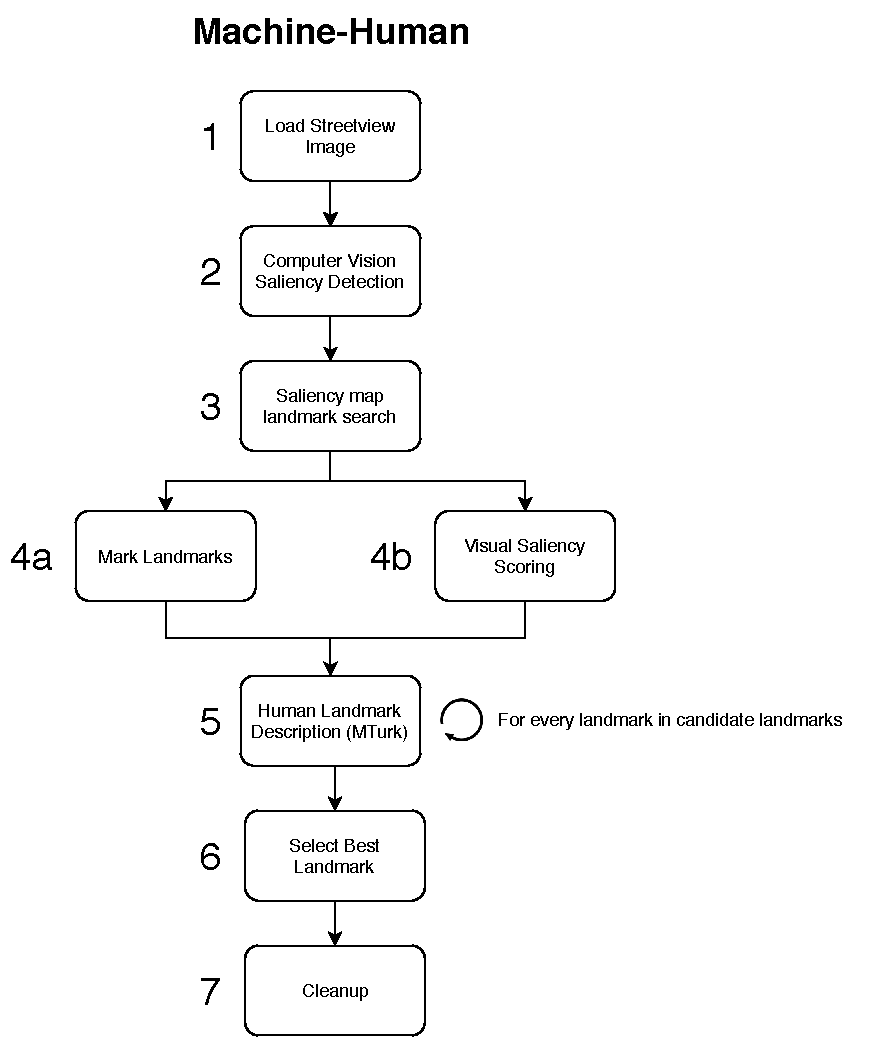
\includegraphics[width=0.6\textwidth]{pipeline_diagrams/machine-human.pdf}
  \caption{The pipeline structure of the Machine-Human pipeline.}
  \label{fig:pipeline:mh}
\end{figure}

\subsubsection*{Step 1: Load Streetview Image}
\textbf{Input}: $X_1 = X_0 = (latitude, longitude, bearing)$
\textbf{Output}: $Y_1 = (latitude, longitude, bearing, [image_urls])$

This step is implemented in the same manner as Step 1 of the Machine-Machine pipeline.

\subsubsection*{Step 2: Computer Vision Saliency Detection}
\textbf{Input}: $X_2 = Y_0 = (latitude, longitude, bearing, [image_urls])$
\textbf{Output}: $Y_2 = (latitude, longitude, bearing, [image_urls], [saliency_matrices])$ 

This step is implemented in the same manner as Step 2a of the Machine-Machine pipeline.

\subsubsection*{Step 3a: Create annotated maneuver point images}
\textbf{Input}: $X_{3a} = Y_2 = (latitude, longitude, bearing, [image_urls], [saliency_matrices])$ 
\textbf{Output}: $Y_{3a} = (latitude, longitude, bearing, [image_urls], [saliency_matrices], [annotated_image_urls])$ 

In order for human workers to provide written descriptions for candidate landmarks, they need to see an image of the maneuver point with the candidate landmark outlined. We choose to show workers an annotated image of the entire maneuver point, as opposed to a cropped image containing only the candidate landmark, so that workers can incorporate context into their descriptions. For example, we have observed descriptions such as “one story blue house next to the oak tree” and “stop sign near the crosswalk”.

For each candidate $c$ in the set of candidate landmarks $C$, we generate an image which contains a 3-pixel thick red border drawn around the bounding box of $c$. These images are stored on S3, and the URLs are included in the output of this step.

\subsubsection*{Step 3b: Visual Saliency Scoring}

\textbf{Input}: $X_{3b} = Y_2 = (latitude, longitude, bearing,  [image_urls], [saliency_maps], [candidate_landmarks] )$
\textbf{Output}: $Y_{3b} = (latitude, longitude, bearing,  [image_urls], [candidate_landmarks] )$ 

This step is implemented in the same manner as Step 3 of the Machine-Machine pipeline, except that the landmark search (watershed) component is not needed as all candidate landmarks include bounding boxes.

\subsubsection*{Step 4: Human-based Landmark Description}

\textbf{Input}: $X_4 = Y_{3a} \cup Y_{3b} = (latitude, longitude, bearing, [image_urls], [saliency_matrices], [annotated_image_urls])$ 
\textbf{Output}: $Y_4 = (latitude, longitude, bearing, [image_urls], [saliency_matrices], [annotated_image_urls])$ 

For each landmark $c$ in the set of candidate landmarks $C$, we utilize the human-based description method described in the Saliency section to obtain a lexical description of $c$. These descriptions are included in the given candidate landmark tuple in the output of this step. This step does not complete until all candidate landmarks have been processed through MTurk.

\subsubsection*{Step 5: Select Most Salient Landmark}

\textbf{Input}: $X_5 = Y_4 = (latitude, longitude, bearing,  [image_urls], [saliency_maps], [candidate_landmarks] )$
\textbf{Output}: $Y_5 = (latitude, longitude, bearing, best_landmark)$
 
This step is implemented in the same manner as Step 4 of the Machine-Machine pipeline.

\subsubsection*{Step 6: Cleanup}

\textbf{Input}: $X_6 = Y_5 = (latitude, longitude, bearing, best_landmark)$
\textbf{Output}: $Y_6 = (best_landmark)$

This step is implemented in the same manner as Step 5 of the Machine-Machine pipeline.

\subsection{Human-Human}
\textbf{Input}: $X_0 = (latitude, longitude, bearing)$
\textbf{Output}: The most salient landmark, including a description for use in navigation instructions
\textbf{Candidate selection}: Description

\begin{figure}[htbp]
  \centering
  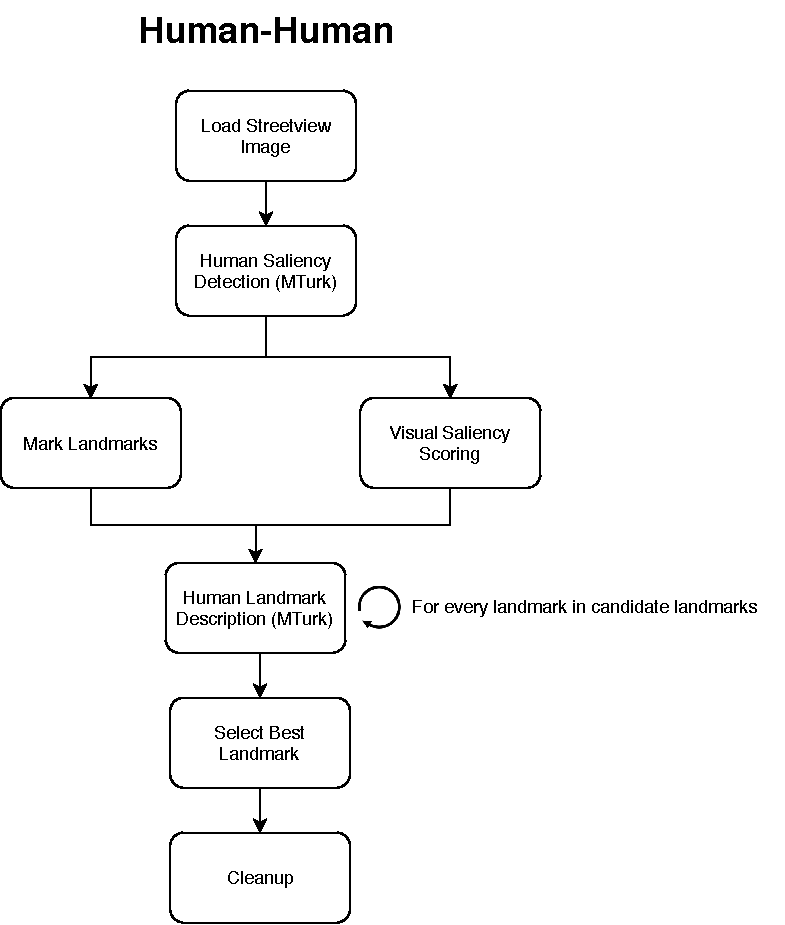
\includegraphics[width=0.6\textwidth]{pipeline_diagrams/human-human.pdf}
  \caption{The pipeline structure of the Human-Human pipeline.}
  \label{fig:pipeline:hh}
\end{figure}

\subsubsection*{Step 1: Load Streetview Image}
\textbf{Input}: $X_1 = X_0 = (latitude, longitude, bearing)$
\textbf{Output}: $Y_1 = (latitude, longitude, bearing, [image_urls])$

This step is implemented in the same manner as Step 1 of the Machine-Machine pipeline.

\subsubsection*{Step 2: Human Saliency Detection} 
\textbf{Input}: $X_{2} = Y_1 = (latitude, longitude, bearing, [image_urls])$
\textbf{Output}: $Y_{2} = (latitude, longitude, bearing, [image_urls], [saliency_matrices])$ 

This step is implemented in the same manner as Step 2a of the Human-Machine pipeline.

\subsubsection*{Step 3a: Create annotated maneuver point images}
\textbf{Input}: $X_{3a} = Y_2 = (latitude, longitude, bearing, [image_urls], [saliency_matrices])$ 
\textbf{Output}: $Y_{3a} = (latitude, longitude, bearing, [image_urls], [saliency_matrices], [annotated_image_urls])$ 

This step is implemented in the same manner as Step 3a of the Machine-Human pipeline.

\subsubsection*{Step 3b: Visual Saliency Scoring}

\textbf{Input}: $X_{3b} = Y_2 = (latitude, longitude, bearing,  [image_urls], [saliency_maps], [candidate_landmarks] )$
\textbf{Output}: $Y_{3b} = (latitude, longitude, bearing,  [image_urls], [candidate_landmarks] )$ 

This step is implemented in the same manner as Step 3 of the Machine-Machine pipeline, except that the landmark search (watershed) component is not needed as all candidate landmarks include bounding boxes.

\subsubsection*{Step 4: Human-based Landmark Description}

\textbf{Input}: $X_4 = Y_{3a} \cup Y_{3b} = (latitude, longitude, bearing, [image_urls], [saliency_matrices], [annotated_image_urls])$ 
\textbf{Output}: $Y_4 = (latitude, longitude, bearing, [image_urls], [saliency_matrices], [annotated_image_urls])$ 

This step is implemented in the same manner as Step 4 of the Machine-Human pipeline.

\subsubsection*{Step 5: Select Most Salient Landmark}

\textbf{Input}: $X_5 = Y_4 = (latitude, longitude, bearing,  [image_urls], [saliency_maps], [candidate_landmarks] )$
\textbf{Output}: $Y_5 = (latitude, longitude, bearing, best_landmark)$
 
This step is implemented in the same manner as Step 4 of the Human-Machine pipeline.

\subsubsection*{Step 6: Cleanup}

\textbf{Input}: $X_6 = Y_5 = (latitude, longitude, bearing, best_landmark)$
\textbf{Output}: $Y_6 = (best_landmark)$

This step is implemented in the same manner as Step 5 of the Machine-Machine pipeline.



